\documentclass[UTF8,a4paper,10pt, twocolumn]{ctexart}
\usepackage[left=2.50cm, right=2.50cm, top=2.50cm, bottom=2.50cm]{geometry}

% -- text font --
% compile using Xelatex

%\setmainfont{Microsoft YaHei}  % 微软雅黑
%\setmainfont{YouYuan}  % 幼圆
%\setmainfont{NSimSun}  % 新宋体
%\setmainfont{KaiTi}    % 楷体
%\setmainfont{SimSun}   % 宋体
%\setmainfont{SimHei}   % 黑体

\usepackage{times} 
%\usepackage{mathpazo}
%\usepackage{fourier}
%\usepackage{charter}
%\usepackage{helvet}

\usepackage{amsmath, amsfonts, amssymb} % math equations, symbols
\usepackage[english]{babel}
\usepackage{color}      % color content
\usepackage{graphicx}   % import figures
\usepackage{url}        % hyperlinks
\usepackage{bm}         % bold type for equations
\usepackage{multirow}
\usepackage{booktabs}
\usepackage{epstopdf}
\usepackage{epsfig}
\usepackage{algorithm}
\usepackage{algorithmic}
\usepackage{stfloats}
\renewcommand{\algorithmicrequire}{ \textbf{Input:}}     % use Input in the format of Algorithm
\renewcommand{\algorithmicensure}{ \textbf{Initialize:}} % use Initialize in the format of Algorithm
\renewcommand{\algorithmicreturn}{ \textbf{Output:}}     % use Output in the format of Algorithm

\usepackage{fancyhdr}   % 设置页眉、页脚
%\pagestyle{fancy}
\lhead{}
\chead{}
\lfoot{}
\cfoot{}
\rfoot{}

% \usepackage{draftwatermark}         % 所有页加水印
% %\usepackage[firstpage]{draftwatermark} % 只有第一页加水印
% \SetWatermarkText{Water-Mark}           % 设置水印内容
% \SetWatermarkText{\includegraphics{fig/ZJDX-WaterMark.eps}}         % 设置水印logo
% \SetWatermarkLightness{0.9}             % 设置水印透明度 0-1
% \SetWatermarkScale{1}                   % 设置水印大小 0-1

% \usepackage{hyperref}   % bookmarks
% \hypersetup{colorlinks, bookmarks, unicode} % unicode


\title{密码学技术与区块链}
\author{ SA18225036 陈旻 }
\date{}

\begin{document}
    \maketitle
    \thispagestyle{fancy}
\section{概述} \label{sec:one}
自2009年比特币首次亮相以来,其基础技术-区块链已经展现了良好的应用前景,引起了学术界和业界的广泛关注。作为第一个加密货币,比特币被评为2015年表现最好的货币和2016年表现最佳的商品。与此同时,区块链技术已应用于许多领域,包括医学、经济学、物联网、软件工程等。引入图灵完整的编程语言,使用户能够开发在区块链上运行的智能合约,标志着区块链2.0时代的开始。利用区块链的分布式共识机制,智能合约允许相互不信任的用户完成数据交换或交易,而无需任何第三方信任机构。以太坊现在成为使用最广泛的基于区块链的智能合约。区块链技术是多种底层技术的融合,主要包括:点对点网络技术、密码学技术、块链式结构和共识算法等等。虽然智能合约并不是区块链系统的必要组成部分,但由于区块链具备不可篡改、规则透明、多方执行等特性,使它可以很好地为智能合约提供可信的计算环境.因此,我们首先对4种典型区块链技术框架进行介绍,然后从区块数据结构、密码学、共识机制、智能合约等方面进行对比,分析存在的安全问题。

\section{区块链基础构架及加密技术} \label{sec:two}
\subsection{区块链基础构架}
区块链技术的基础架构模型如图2 所示。一般说来, 区块链系统由数据层、网络层、共识层、激励层、合约层和应用层组成。其中, 数据层封装了底层数据区块以及相关的数据加密和时间戳等技术; 网络层则包括分布式组网机、数据传播机制和数据验证机制等; 共识层主要封装网络节点的各类共识算法; 激励层将经济因素集成到区块链技术体系中来, 主要包括经济激励的发行机制和分配机制等; 合约层主要封装各类脚本、算法和智能合约, 是区块链可编程特性的基础; 应用层则封装了区块链的各种应用场景和案例。该模型中, 基于时间戳的链式区块结构、分布式节点的共识机制、基于共识算力的经济激励和灵活可编程的智能合约是区块链技术最具代表性的创新点。
\begin{figure}[htbp]
	\centering
	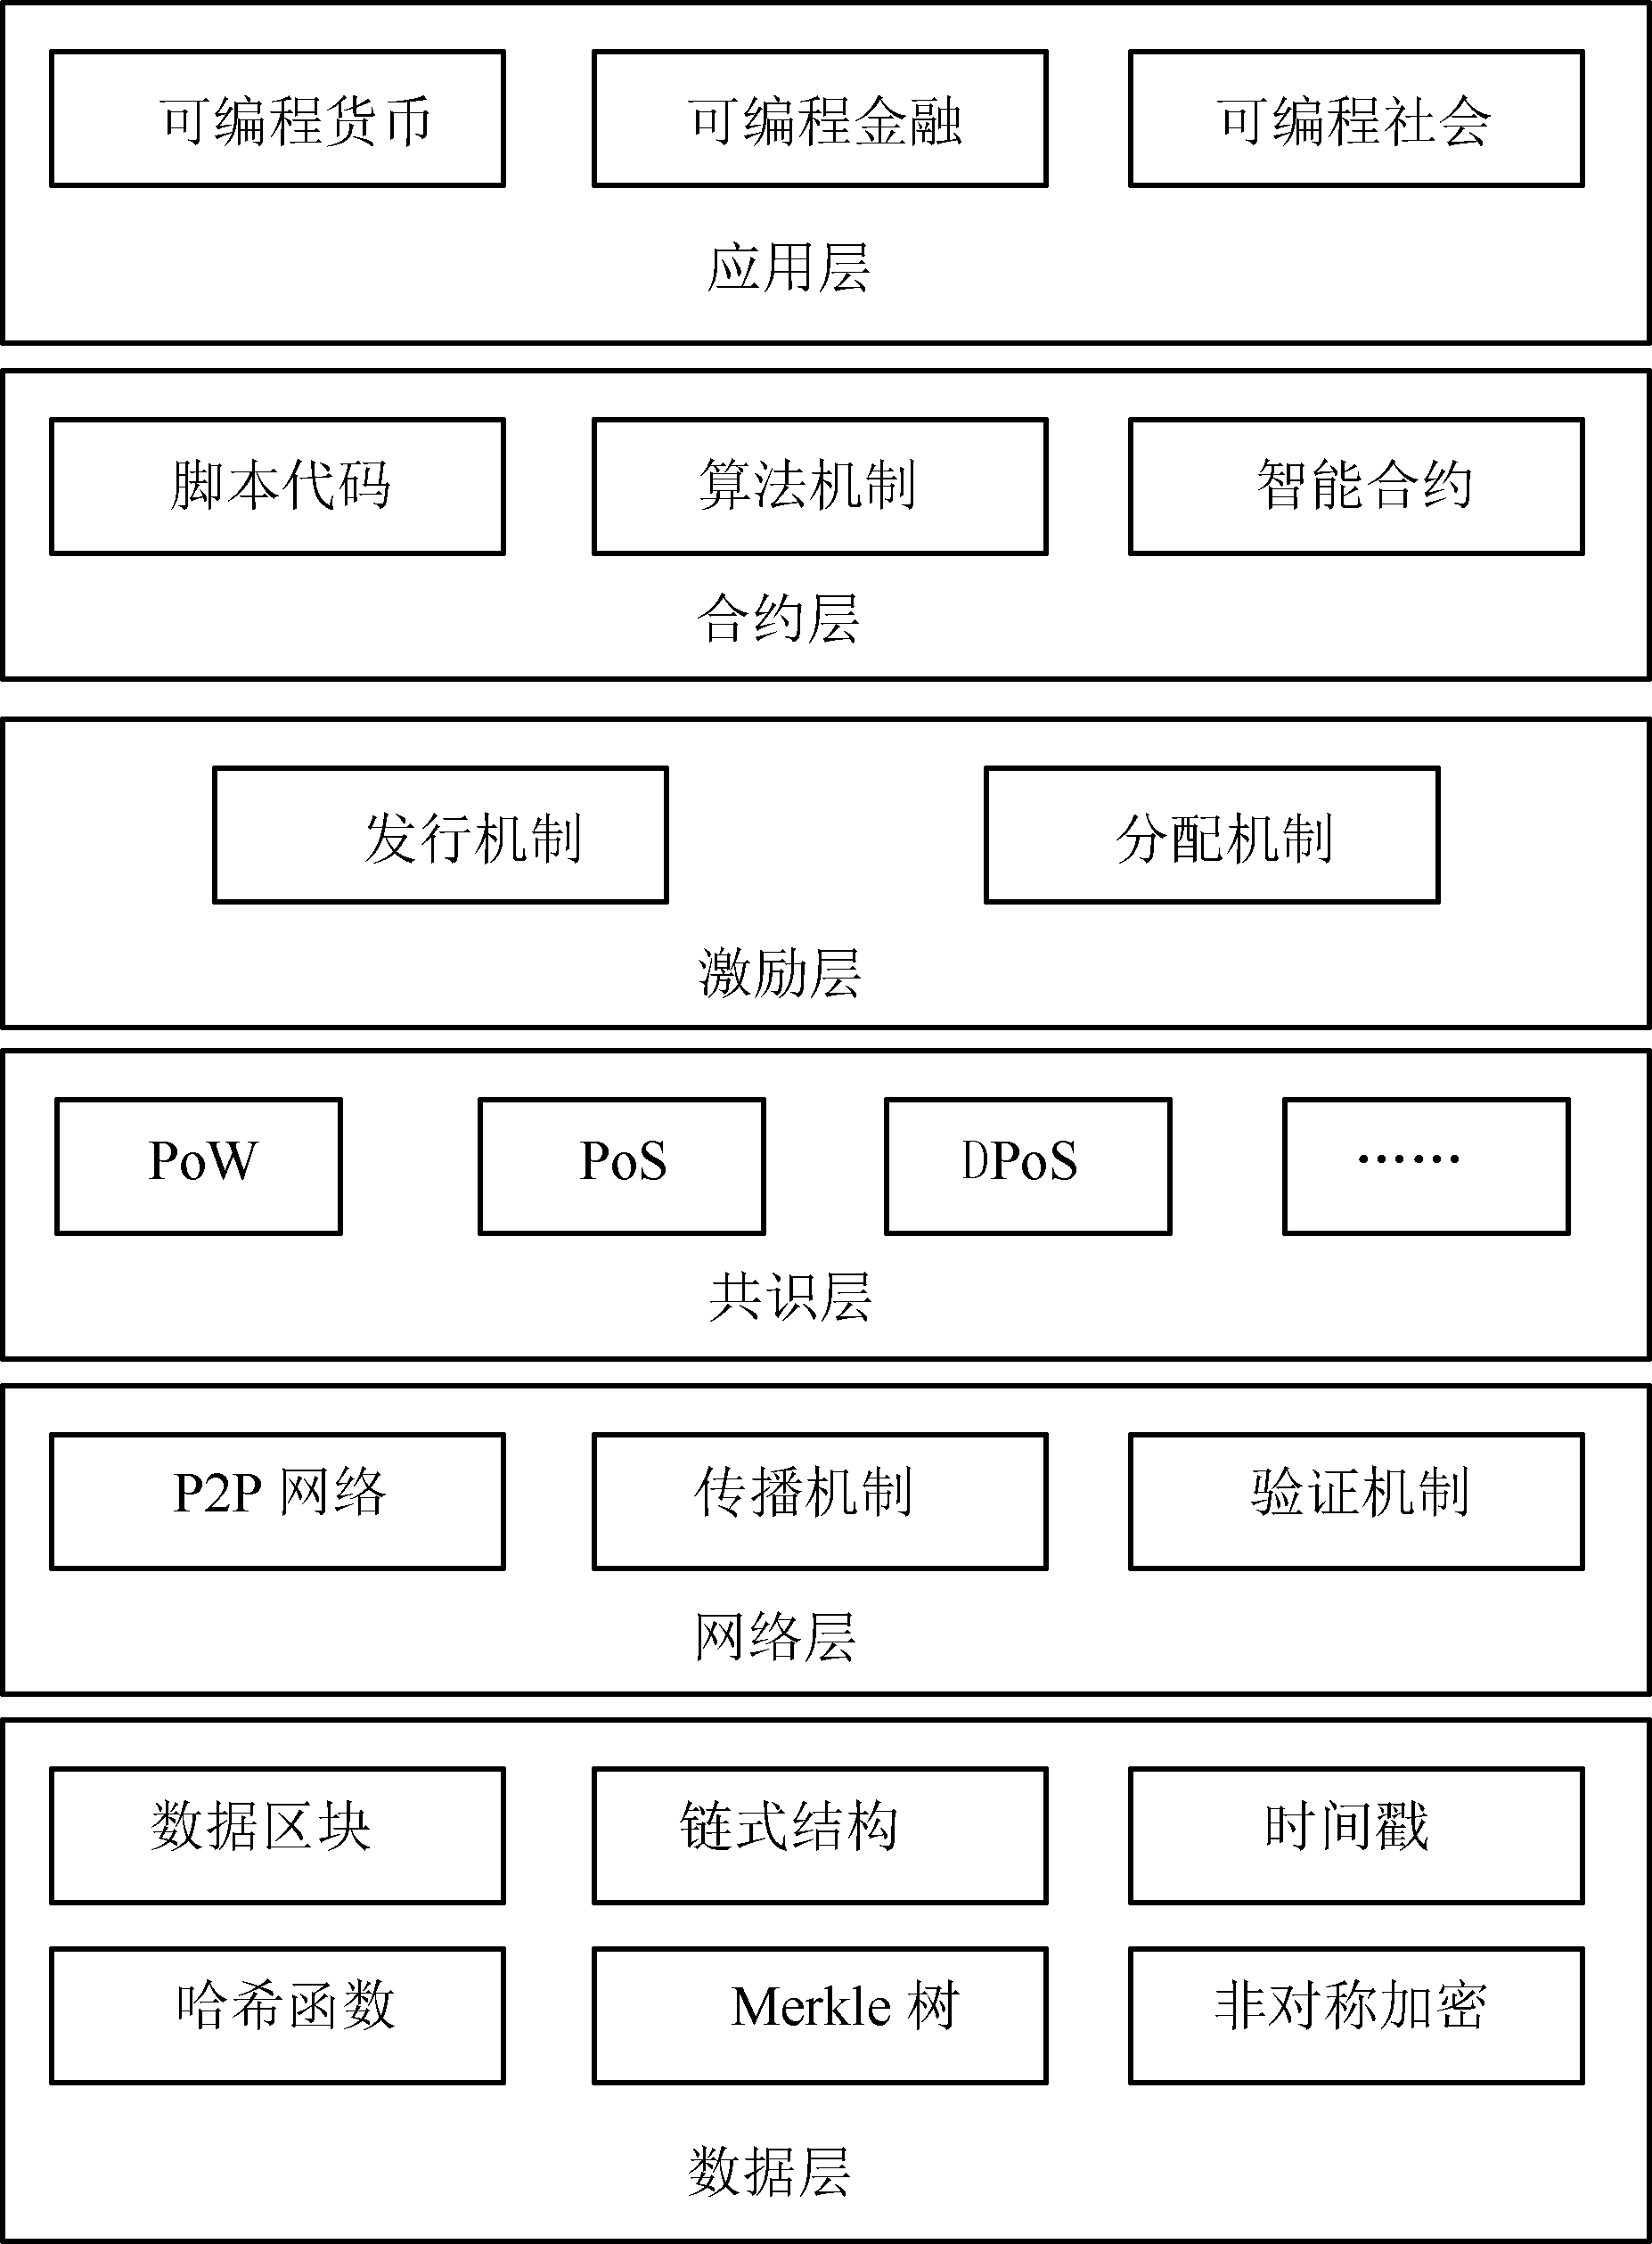
\includegraphics[width=0.4\textwidth]{fig/basearc.png}
	\caption{区块链基础架构模型}
\end{figure}

\subsection{基础加密技术}
区块链中的加密技术主要应用于数据层。狭义的区块链即是去中心化系统各节点共享的数据账本。 每个分布式节点都可以通过特定的哈希算法和Merkle 树数据结构, 将一段时间内接收到的交易数据和代码封装到一个带有时间戳的数据区块中, 并链接到当前最长的主区块链上, 形成最新的区块。 该过程涉及区块、链式结构、哈希算法、Merkle树和时间戳等技术要素。下面主要对其中的哈希函数和非对称加密过程进行介绍。
\paragraph{哈希函数}
区块链通常并不直接保存原始数据或交易记录, 而是保存其哈希函数值, 即将原始数据编码为特定长度的由数字和字母组成的字符串后记入区块链。 哈希函数(也称散列函数) 具有诸多优良特点, 因而特别适合用于存储区块链数据。例如, 通过哈希输出几乎不能反推输入值(单向性), 不同长度输入的哈希过程消耗大约相同的时间(定时性) 且产生固定长度的输出(定长性), 即使输入仅相差一个字节也会产生显著不同的输出值(随机性) 等。比特币区块链通常采用双SHA256 哈希函数, 即将任长度的原始数据经过两次SHA256 哈希运算后转换为长度为256 位(32 字节) 的二进制数字来统一存储和识别。 除上述特点外, SHA256 算法还具有巨大的散列空间(2256) 和抗碰撞(避免不同输入值产生相同哈希值) 等特性, 可满足比特币的任何相关标记需要而不会出现冲突。
\begin{figure}[htbp]
	\centering
	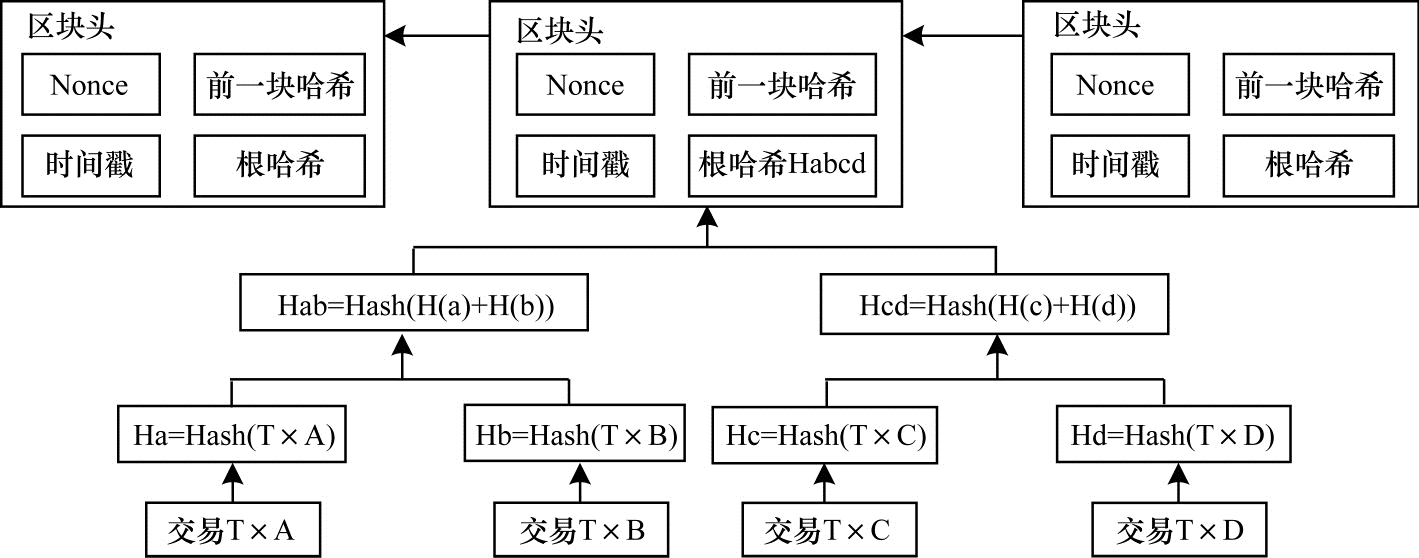
\includegraphics[width=0.4\textwidth]{fig/hash.png}
	\caption{区块数据结构}
\end{figure}
\begin{table*}[hb]
	\caption{典型哈希算法比较} \label{tab:table}
	\centering
	\addtolength{\tabcolsep}{-0mm} % 控制列间距
	\begin{tabular}{cccc}
		\toprule[0.75pt]	% package booktabs
		加密算法 & 安全性 & 运算数的 & 输出大小/b \\
		\midrule[0.5pt]	% package booktabs
		MD5 & 低 & 快 & 128 \\  % package multirow
		SHA1 & 中 & 中 & 160 \\
		SHA256 & 高 & 比SHA1略低 & 256 \\
		SM3 & 高 & 比SHA1略低 & 256 \\
		\bottomrule[0.75pt]	% package booktabs
	\end{tabular}
\end{table*}
\paragraph{非对称加密}
非对称加密是为满足安全性需求和所有权验证需求而集成到区块链中的加密技术,常见算法包括RSA、Elgamal、Rabin、D-H、ECC(即椭圆曲线加密算法) 等。 非对称加密通常在加密和解密过程中使用两个非对称的密码, 分别称为公钥和私钥。 非对称密钥对具有两个特点, 首先是用其中一个密钥(公钥或私钥) 加密信息后, 只有另一个对应的密钥才能解开; 其次是公钥可向其他人公开、私钥则保密, 其他人无法通过该公钥推算出相应的私钥。 非对称加密技术在区块链的应用场景主要包括信息加密、数字签名和登录认证等, 其中信息加密场景主要是由信息发送者(记为A) 使用接受者(记为B) 的公钥对信息加密后再发送给B, B 利用自己的私钥对信息解密。 比特币交易的加密即属于此场景; 数字签名场景则是由发送者A 采用自己的私钥加密信息后发送给B, B 使用A 的公钥对信息解密、从而可确保信息是由A 发送的; 登录认证场景则是由客户端使用私钥加密登录信息后发送给服务器, 后者接收后采用该客户端的公钥解密并认证登录信息。以比特币系统为例, 其非对称加密机制如图4所示: 比特币系统一般通过调用操作系统底层的随机数生成器来生成256 位随机数作为私钥。 比特币私钥的总量可达2256, 极难通过遍历全部私钥空间来获得存有比特币的私钥, 因而是密码学安全的。为便于识别, 256 位二进制形式的比特币私钥将通过SHA256 哈希算法和Base58 转换, 形成50 个字符长度的易识别和书写的私钥提供给用户; 比特币的公钥是由私钥首先经过Secp256k1 椭圆曲线算法生成65 字节长度的随机数。 该公钥可用于产生比特币交易时使用的地址, 其生成过程为首先将公钥进行SHA256 和RIPEMD160 双哈希运算并生成20 字节长度的摘要结果(即hash160 结果), 再经过SHA256 哈希算法和Base58 转换形成33 字符长度的比特币地址。 公钥生成过程是不可逆的, 即不能通过公钥反推出私钥。 
\subsection{隐私保护}
区块链系统要实现隐私保护,离不开密码学的支撑。无论是采用UTXO 模型,还是采用账户模型,在许多区块链系统中所有的交易数据是公开保存的,通过追踪和分析地址间的交易记录,可以推测出用户身份。为了提高区块链技术的匿名性,保护用户的身份隐私,多种区块链隐私保护方案被提出。

在混币协议中,不同用户被要求同时将相同金额发送到混合服务器,服务器对交易内容混合处理后,将比特币发送到用户新地址。资金经过混合处理后,隐藏了交易输入、输出地址的直接联系,使得攻击者对交易内容的分析变得困难,从而保证用户的隐私。

门罗币、零币、零钞等均基于加密协议实现隐私保护。门罗币基于CryptoNote协议,通过环签名和隐蔽地址的方式来隐藏输入输出地址之间的关联,环签名技术保证了交易的隐私。后人提出一种基于零知识证明的加密协议,即零币。零币是比特币的一种扩展协议,比特币用户可以通过该协议将比特币转化为零币,从而隐藏交易的输入、输出地址。其他用户只能知道零币是否被花费,而无法获取其余的交易信息。之后在零币的基础上发展出了零钞,将加密技术提高到了更高的层次。零钞使用了zk-SNARK技术,该技术可以使零知识证明更加简洁。与零币相比,零钞中的交易金额也是保密的,并且可以将不同面值的币铸造成多个等值的币。

由于区块链交易的速度原因,因此一些依赖第三方的链下达成交易方案被提出,这些方案也称为安全通道协议。在安全通道协议的技术框架下,Lightning Network、Sprites、Bolt、TumbleBit等技术致力于解决存在第三方时的隐私安全问题。常见隐私保护技术的性能对比结果见表1。

\begin{table*}[hb]
	\caption{隐私保护技术的性能对比结果} \label{tab:table}
	\centering
	\addtolength{\tabcolsep}{-0mm} % 控制列间距
	\begin{tabular}{ccccc}
		\toprule[0.75pt]	% package booktabs
		名称 & 核心技术 & 特点 & 结构 & 隐私保护效果 \\
		\midrule[0.5pt]	% package booktabs
		比特币 & 签名验签 & 公钥作为身份,私钥私有 & 去中心化 & 差 \\  % package multirow
		门罗币 & 环签名 & 采用环签名的方式实现地址隐私保护 & 去中心化 & 好 \\
		零币 & 零知识证明 & 隐藏交易信息 & 去中心化 & 好 \\
		零钞 & 零知识证明 & 隐藏交易信息、交易金额 & 去中心化 & 好 \\
		盲币 & 盲签名 & 匿名性取决于第三方混币服务 & 中心化 & 好 \\
		EOS & 多签名 & 通过多签名可以起到投票的作用 & 去中心化 & 好 \\
		\bottomrule[0.75pt]	% package booktabs
	\end{tabular}
\end{table*}

\section{加密技术的原理及比较} \label{sec:two}
本文主要对非对称加密技术进行原理介绍和比较非对称加密主要算法有:RSA、Elgamal、背包算法、Rabin、D-H、ECC(椭圆曲线加密算法)等;非对称加密拥有两个密钥:公开密钥(publickey)和私有密钥(privatekey)。
\subsection{RSA算法}
RSA算法是当前最著名、应用最广泛的公钥系统,1978年由美国麻省理工学院的Ron Rivest、 Adi Shamir 和Leonard Adleman在论文《获得数字签名和公开钥密码系统的方法》中提出的。这是一个基于数论的非对称(公开钥)密码体制,采用分组加密方式。其名称来自于三个发明者的姓名首字母。它的安全性是基于大整数素因子分解的困难性,而大整数因子分解问题是数学上的著名难题,至今没有有效的方法予以解决,因此可以确保RSA算法的安全性。RSA系统是公钥系统的最具有典型意义的方法,大多数使用公钥密码进行加密和数字签名的产品和标准使用的都是RSA算法。

RSA算法是第一个既能用于数据加密也能用于数字签名的算法,因此它为公用网络上信息的加密和鉴别提供了一种基本的方法。它通常是先生成一对RSA 密钥,一个是保密密钥,由用户保存;另一个为公开密钥,可对外公开,甚至可在网络服务器中注册,人们用公钥加密文件发送给个人,个人就可以用私钥解密接收。为提高保密强度,RSA密钥一般为1024或者2048位。

\begin{algorithm}
	\caption{RSA算法的工作原理}
	\begin{algorithmic}[1]
		\ENSURE 任意选取两个不同的大质数p和q\\           % this command shows "Initialized"
		
		\STATE 计算乘积$r=p*q$ \\  % line number at left side
		\STATE 任意选取一个大整数e,e与$(p-1)*(q-1)$互质,整数e用做加密密钥。注意:e的选取是很容易的,所有大于p和q的质数都可用 \\
		\STATE 确定解密密钥d: $d * e = 1 \mod{(p - 1)*(q - 1)}$根据e、p和q可以容易地计算出d \\
		\STATE 公开整数r和e,但是不公开d \\
		\STATE 将明文P(P是一个小于r的整数)加密为密文C,$ C = P^e \mod r$ \\
		\STATE 将密文C解密为明文P,$P = C^d \mod r$

	\end{algorithmic}
\end{algorithm}

RSA算法解决了大量网络用户密钥管理的难题,这是公钥密码系统相对于对称密码系统最突出的优点。但是它同时也存在一定的缺点:
\begin{enumerate}
\item 产生密钥很麻烦,受到素数产生技术的限制,因而难以做到一次一密。
\item 安全性。RSA的安全性依赖于大数的因子分解,但并没有从理论上证明破译RSA的难度与大数分解难度等价。目前,人们已能分解140多个十进制位的大素数,这就要求使用更长的密钥,速度更慢;另外,目前人们正在积极寻找攻击RSA的方法,如选择密文攻击,一般攻击者是将某信息伪装(Blind),让拥有私钥的实体签署。然后,经过计算就可得到它所想要的信息。实际上,攻击利用的都是同一个弱点,即存在这样一个事实:乘幂保留了输入的乘法结构: $ (XM)_d = X_d *M_d \mod n$。前面已经提到,这个固有的问题来自于公钥密码系统的最有用的特征:每个人都能使用公钥。但从算法上无法解决这一问题,主要措施有两条:一条是采用好的公钥协议,保证工作过程中实体不对其他实体任意产生的信息解密,不对自己一无所知的信息签名;另一条是决不对陌生人送来的随机文档签名,签名时首先使用One-Way Hash Function对文档作HASH处理,或同时使用不同的签名算法。除了利用公共模数,人们还尝试一些利用解密指数或$\Phi (n)$等攻击。
\item 速度慢。由于RSA 的分组长度太大,使运算代价很高,尤其是速度较慢,较对称密码算法慢几个数量级;且随着大数分解技术的发展,这个长度还在增加,不利于数据格式的标准化。目前,SET(Secure Electronic Transaction)协议要求CA采用2048比特的密钥,其他实体使用1024比特的密钥。为了速度问题,目前人们广泛采取单、公钥密码结合使用的方法,优缺点互补:单钥密码加密速度快,人们用它来加密较长的文件,然后用RSA给文件密钥加密,极好地解决了单钥密码的密钥分发问题。
\end{enumerate}

\subsection{DSA算法}
DSA(Digital Signature Algorithm,数字签名算法)是Schnorr和ElGamal签名算法的变种,被美国NIST作为DSS(DigitalSignature Standard,数字信号标准)。DSA算法是基于整数有限域离散对数难题的,其安全性与RSA相似。DSA的一个重要特点是两个素数公开,这样,当使用别人的p和q时,即使不知道私钥,也能确认它们是否是随机产生的,还是作了手脚。RSA算法却做不到。

安全性 
DSA主要依赖于整数有限域离散对数难题。素数 P 必须足够大,且p-1至少包含一个大素数因子以抵抗Pohlig \& Hellman算法的攻击。M一般都应采用信息的HASH值(官方推荐为SHA算法)。DSA的安全性主要依赖于p和g,若选取不当则签名容易伪造,应保证g对于p-1的大素数因子不可约。个人认为:DSA的安全性要次于ECC, 与RSA不相上下。但是,在DSA算法的验证过程中, R和S 是以明文形式出现的,这点很容易被恶意攻击者利用。

DSA算法在破解时关键的参数就是X,根据 $Y = G^X \mod P$ ,只要知道 P,G,Y,Q 且能分解出 X ,就可以伪造R、S,从而写出KeyGen了。

\subsection{ECC算法}

ECC(Elliptic Curve Cryptosystem,椭圆曲线密码体制)算法中,椭圆曲线指的是由韦尔斯特拉斯(Weierstrass)方程所确定的平面曲线。如下:

$$ y^2 + a_1 xy + a_3 y = x^3 + a_2 x^2 + a_4 x + a_6 $$

若F是一个域$(a_i \in F,i=1,2,…,6)$,且满足式的数偶(x,y)称为F域上的椭圆曲线E的点。F域可以是有理数域,还可以是有限域$GF(Pr)$。椭圆曲线通常用E表示。除了曲线E包含的点,还有一个无穷远点O。

在ECC中,利用了定义在有限域上的椭圆曲线。其方程如下:

$$ 4a^3 + 27b^2(\mod p) \neq 0 $$

这里p是素数,a和b为两个小于p的非负整数。满足式的点(x,y)和一个无穷点O就组成了椭圆曲线E。

椭圆曲线离散对数问题ECDLP定义如下:

给定素数p和椭圆曲线E,对 Q=kP,在已知P,Q的情况下求出小于p的正整数k。可以证明,已知k和P计算Q比较容易,而由Q和P计算k则比较困难,至今没有有效的方法来解决这个问题,这就是ECC原理之所在。

ECC与RSA相比,有以下的优点:
\begin{enumerate}
\item 安全性能更高。如160位ECC与1024位RSA、DSA有相同的安全强度。
\item 计算量小,处理速度快。在私钥的处理速度上(解密和签名),ECC远 比RSA、DSA快得多。
\item 存储空间占用小。ECC的密钥尺寸和系统参数与RSA、DSA相比要小得多, 所以占用的存储空间小得多。
\item 带宽要求低。
\end{enumerate}

\subsection{Diffie-Hellman算法}

由于该算法本身限于密钥交换的用途,许多商用产品用做密钥交换技术,因此该算法通常称为Diffie-Hellman密钥交换算法。这种密钥交换技术的目的在于使得两个用户安全地交换一个秘密密钥以便用于以后的报文加密。

Diffie-Hellman密钥交换算法的有效性依赖于计算离散对数的难度。离散对数的定义如下:

首先定义一个素数p的原根,为其各次幂产生从1 到p-1的所有整数根,也就是说,如果a是素数p的一个原根,那么数值
$$ a \mod p, a_2 \mod p, ..., a_{p-1} \mod p $$
是各不相同的整数,并且以某种排列方式组成了从1到p-1的所有整数。

对于一个整数b和素数p的一个原根a,可以找到惟一的指数i,使得
$$ b = a_i \mod p     S.t. 0 \leq i \leq(p-1) $$
指数i称为b的以a为基数的模p的离散对数或者指数。该值被记为inda ,p(b)。

基于此背景知识,可以定义Diffie-Hellman密钥交换算法。该算法描述如下:
1)有两个全局公开的参数,一个素数Q和一个整数A,A是Q的一个原根。

2)假设用户A和B希望交换一个密钥,用户A选择一个作为私有密钥的随机数XA < Q,并计算公开密钥YA=AXA mod Q。A对XA的值保密存放而使YA能被B公开获得。类似地,用户B选择一个私有的随机数$ XB \le Q $,并计算公开密钥YB=AXB mod Q。B对XB的值保密存放而使YB能被A公开获得。

3)用户A产生共享秘密密钥的计算方式是K = (YB)XA mod Q。同样,用户B产生共享秘密密钥的计算是K = (YA)XB mod Q。这两个计算产生相同的结果:
\begin{align}
	K &= (YB)XA \mod Q \\
	&= (AXB \mod Q)XA \mod Q \\
	&= (AXB)XA \mod Q \\
	&= AXBXA \mod Q \\
	&= (aXA)XB \mod q \\
	&= (AXA \mod Q)XB \mod Q \\
	&= (YA)XB \mod q
\end{align}
因此相当于双方已经交换了一个相同的秘密密钥。

4) 因为XA和XB是保密的,一个敌对方可以利用的参数只有Q、A、YA和YB。因而敌对方被迫取离散对数来确定密钥。例如,要获取用户B的秘密密钥,敌对方必须先计算
$$  XB = indA ,Q(YB) $$
然后再使用用户B采用的同样方法计算其秘密密钥K。

Diffie-Hellman密钥交换算法的安全性依赖于这样一个事实:虽然计算以一个素数为模的指数相对容易,但计算离散对数却很困难。对于大的素数,计算出离散对数几乎是不可能的。

\section{隐私保护未来挑战}
区块链被认为是非常安全的,因为用户只进行生成的交易 地址而非真实身份。用户也可以生成许多地址 信息泄漏。但是,区块链不能保证交易隐私,因为每个公钥的所有交易和余额的值都是公开可见。此外,用户的比特币交易 可以链接以显示用户的信息。攻击者可通过获得网络中节点IP 的相关信息关联个人,以及追溯交易对其进行大数据处理可以得到很多有价值的信息,由于用户使用不当会造成DAPP的隐私泄露,可见隐私保护问题亟待加强。第2章介绍了一些密码与隐私保护相关的问题,如用零知识证明解决交易隐藏的问题,用环签名实现地址隐蔽和交易隐蔽。同态加密是指对经过加密的数据进行处理得到一个输出,将该输出进行解密,其结果与用同一方法处理未加密的原始数据得到的输出结果是一样的,这就为密文搜索提供了技术保证,对于交易隐私保护有借鉴意义。安全多方计算解决了一组互不信任的参与方之间保护隐私的协同计算问题,同时不泄露各输入值给参与计算的其他成员。其他形式的零知识证明等密码算法有待进一步实现区块链技术各环节中的隐私保护。此外,基于身份的密码、基于属性的密码以及分层确定性钱包技术等用于用户身份信息的隐私保护也值得研究和关注。为了保护区块链使用者的权益和降低风险,需要考虑KYC 和AML 问题。ChainAnchor 通过在受限的区块链上添加身份认证和隐私保护层,使得任何人可以读和认证交易,并且只有匿名身份认证过的交易才能被处理。
\subsection{发展趋势}
Biryukov等人提出了一个即使用户在网络后面,也可以将用户假名链接到IP地址的方法 地址转换(NAT)或防火墙。在[19]中,每个客户端都可以由一个唯一标识它连接到的节点集。但是,这个集合可以学习并用于查找原点交易,已经提出了多种方法来改善区块链的匿名性,它大致可分为两种类型:
\paragraph{混合}在区块链中,用户地址是假名的。但它仍然有可能 将地址链接到用户真实身份,因为许多用户使用相同的事务进行交易 经常说话。混合服务是一种提供匿名服务的服务 将资金从多个输入地址转移到多个输出地址。 对于例如,具有地址甲的用户艾丽丝想要向地址乙的鲍勃发送一些资金。 如果艾丽斯直接用输入地址甲和输出地址乙进行交易,那么爱丽丝和鲍勃之间的关系可能会被曝光。所以爱丽丝可以发送资金到值得信赖的中介卡罗尔。然后卡罗尔通过多个输入C1将资金转移给鲍勃, C2,C3等,多个输出D1,D2,B,D3等。鲍勃的地址乙也包含在内 在输出地址中。因此,揭示爱丽丝与鲍勃之间的关系变得更加困难。然而中介可能是不诚实的,并揭示了爱丽丝和鲍勃的私人有目的的信息.Carol也有可能将Alice的资金转给她自己的地址而不是Bob的地址.Mixcoin提供了一种避免的简单方法 不诚实的行为。中间人加密用户的要求,包括资金金额和转账日期及其私钥。然后,如果中介没有转移,这笔钱任何人都可以核实被中介骗了。Coinjoin依赖于中央混音服务器进行随机广播输出地址以防止被盗。受Coinjoin启发,CoinShuffle使用 解密混合网络用于地址改组。
\paragraph{匿名}在Zerocoin中,使用了零知识证明。矿工不必验证具有数字签名的交易,但验证属于列表的币有效的币。付款的来源与交易无关,以防止交易图分析。但它仍然显示付款的目的地和金额.Zerocash有人提出要解决这个问题。在Zerocash交易金额以及用户持有的币价值将被隐藏。
\section{结束语}
从目前来看,区块链技术在安全性方面仍存在诸多问题。区块链的非对称加密机制也将随着数学、密码学和计算技术的发展而变得越来越脆弱,而且随着量子计算等新科技的发展,未来非对称加密算法有可能存在被破解的风险。区块链在私钥使用和保存方面仍存在很大问题,长字节私钥一般通过转换,形成短字符长度形式的私钥,但仍然不方便记忆,而有些区块链是去中心化的,是没有第三方参与的,那么如何安全可靠地保存私钥仍是重要问题。
\end{document}

